\chapter{Estado da Arte} \label{cap:eda}
%2345678901234567890123456789012345678901234567890123456789012345678901234567890

Uma ontologia possui inúmeras utilidades tanto em pesquisa quanto na
indústria. Na pesquisa o foco é uma melhor descrição dos domínio propriamente
dito, enquanto na indústria o foco é a melhor utilização dos recursos de seus
colaboradores. No trabalho de \citet{Gutierrez:2007:OVH:1229160.1229164} existem
excelentes exemplos dos usos possíveis de uma ontologia de humano virtual.
Assim, a primeira seção introduz os modelos psicológicos e explica o modelo de
\citet{ortony1988cse}. Na segunda, apresenta ontologias emocionais
desenvolvidas. A terceira seção descreve os trabalhos com ontologias que visam
descrever o físico ou o mental de um humano virtual.

\section{Modelo Cognitivo Emocional} \label{cap:eda:mce}

Estudos neurológicos recentes \cite{ledoux1998emotional,damasio2004erro}
mostram a importância das emoções na tomada de decisão.
\citet{damasio2004erro} definiu emoção como sendo um estado físico do corpo e
o sentimento sendo a percepção desse estado corporal. Além disso, na psicologia
há diferentes modelos que tentam explicar a afetividade.

\citet{scherer2000tnoe} categorizou esses modelos afetivos em quatro
categorias principais. A primeira categoria, modelos dimensionais, visa
descobrir variáveis que representam eixos das classes emotivas e estabelecem
meios de se mover por esses eixos. Os modelos discretos especificam um
conjunto básico de emoções e especificam regras para que o mecanismo evolua.
Já, a categoria dos baseados em significados se preocupa com as situações
em que o sentimento foi ocasionado e tenta descrever estruturas semânticas dos
mesmos. Por fim, os modelos baseados em componentes entendem que os
sentimentos são aprendidos ao longo do tempo e, sendo assim, estudam o elo
entre os sentimentos e as suas situações. Esse elo é montado de diferentes
formas e varia de pessoa para pessoa.

\begin{figure}[t]
  \centering
    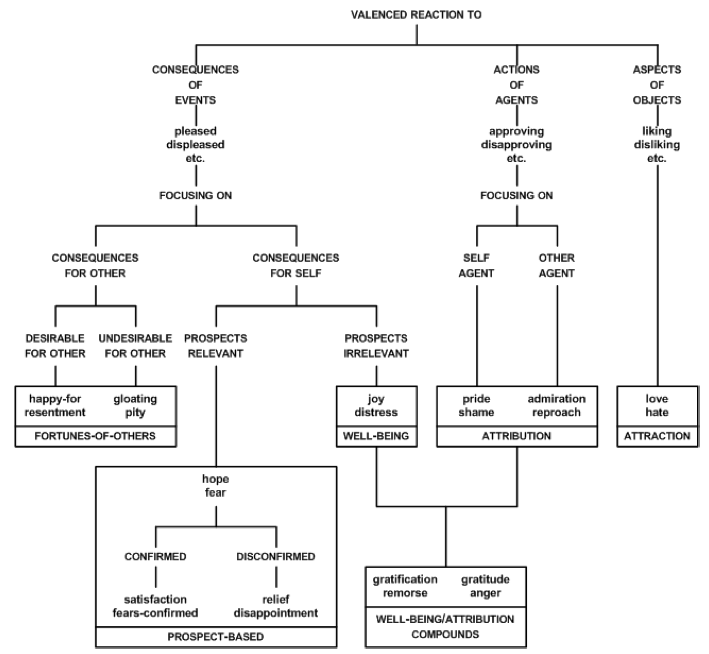
\includegraphics[width=150mm]{figuras/occ.png}
  \caption{Estrutura de emoções \cite{ortony1988cse}.}
  \label{fig:occ_model}
\end{figure}

Um modelo bastante conhecido na Inteligência Artificial foi definido por
\citet{ortony1988cse}. Esse modelo\footnote{A partir daqui o modelo será
referenciado como modelo \occ.} baseado em significados possui 22 emoções
descritas com suas situações. Essas emoções são divididas em
formas de se perceber o mundo a sua volta por consequências (importantes para
alguma meta), ações (julga a responsabilidade) e objetos (atração ou repulsa).
Assim sendo, essas maneiras de se perceber o mundo refletem diferentes jeitos
de se analisar as situações que podem ser relativas aos objetivos, valores
morais ou gostos da pessoa.

A Figura~\ref{fig:occ_model} resume esse modelo e mostra as
percepções possíveis de um indivíduo.  Partindo da direita para esquerda, o
ramo mais básico, \emph{Aspects Of Objects}, é ativado quando se avalia o
gosto de alguém para algum objeto (inanimado ou não). Por exemplo, Millie
gosta de rosas azuis. No seguinte, \emph{Actions Of Agents}, o julgamento das
ações exercidas por outro indivíduo ou por si mesmo é realizado baseado nos
valores morais da pessoa que está julgando. Exemplo: reprovar a atitude dos
bancários que fazem greve a cada ano. Cabe salientar, que ao julgar ações, o
modelo permite um grau de ``empatia'' chamado pelos autores de ``unidade de
força cognitiva''\footnote{Traduzido literalmente de \emph{Strength of
cognitive unit}.}. Dessa forma, é possível, por exemplo, ficar com orgulho
porque uma atleta ganhou uma medalha ou ficar envergonhado ao descobrir que o
vizinho bate no(s) filho(s).

O último ramo da árvore, mais a esquerda na Figura~\ref{fig:occ_model}, é o
\emph{Consequences Of Events} que representa as coisas que aconteceram (e
foram consideradas importantes), acontecem ou acontecerão (objetivos
almejados)\dev{}. Essas emoções são avaliadas segundo as suas consequências
para o alcance ou impedimento dos seus objetivos. A emoção sentida ao receber
uma boa nota em um teste, ao ser assaltado ou ao perceber não ser possível
chegar em um destino planejado são exemplos possíveis desse ramo do modelo.

Toda a emoção do modelo trabalha com duas intensidades. A intensidade da
emoção que representa o físico e a intensidade do sentimento que representa o
quanto o agente esta percebendo daquela emoção. Dessa forma, um indivíduo só
possui sentimento quando a intensidade da emoção ultrapassa um
determinado limite\dev{}.  Essa intensidade é obtida por uma função matemática
que utiliza variáveis de dois tipos: locais, que influenciam as emoções do ramo
específico; e globais, que influênciam todas as emoções do modelo.  Um exemplo
de variável local é o desejo, enquanto que um exemplo de variável global pode
ser o senso de realidade de uma pessoa.

\citet{bates1994role} foi um dos primeiros a trabalhar na utilização de emoções
na área de animação. Nessa área, o estudo do comportamento humano é
realizado visando imitar as ações humanas. A principal afirmativa do trabalho
é que o comportamento emotivo de um personagem é um papel importante para que
o mesmo pareça ter vida própria. Esse trabalho utilizou o modelo descrito
visando melhorar a credibilidade de seus atores. Por exemplo, um dos agentes
lida com o medo sendo agressivo com os outros enquanto outro agente lida com a
mesma emoção sendo retraído.

Visando entender melhor o impacto da emoção na tomada de decisão,
\citet{zhang2009emotional} desenvolveram uma aplicação que os sentimentos
afetam o planejamento das ações à serem realizadas.
\citet{neto2010construction} focaram no mesmo objetivo, porém visando estudar
o impacto da memória no planejamento. Sendo assim, eles fizeram um meio
para o agente ``esquecer'' determinadas crenças quando o estado emocional
for diferente daquele guardado anteriormente. Essa característica torna o
planejamento e as atitudes dos personagens virtuais mais realistas.

O projeto \emph{Relational Agents} de \citet{bick2003relational} possui o
objetivo de possibilitar aos usuários a criação de um relacionamento social e
emocional com longa duração. Com a confiança no agente se torna possível
discutir tarefas mais importantes como melhora da saúde ou até a compra de uma
casa \cite{bickmore2009virtual}. Da mesma forma, o projeto AIDA\footnote{Mais
detalhes, ver \url{http://senseable.mit.edu/aida}.} tem por objetivo entender
o estado afetivo da pessoa dirigindo para tentar sugerir ao usuário mudanças
em suas rotas baseado na rotina aprendida anteriormente. Ambos os trabalhos
podem ser entendidos como enquadrados na área de IHC.

Um dos trabalhos mais conhecidos baseado no modelo \occ é, sem dúvida, o de
\citet{kshirsagar2002multilayer}\todo{falar mais na dissertacao?}. Ele utilizou
as emoções levantadas no modelo em conjunto com um modelo de personalidade
baseado na psicologia que leva em consideração 5 fatores. O primeiro fator,
extroversão, é descrito como a preferência para o comportamento em situações
sociais. O segundo, agradabilidade, é a interação com outros outros
indivíduos. Outro fator é a conscientização que é a organização e persistência
das metas. A tendência de pensamentos negativos é o chamada de fator
neurótico. O último fator é o que descreve se a pessoa tem interesse em
cultura ou é ``cabeça aberta''.

\section{Ontologias Emocionais} \label{cap:eda:oe}

Ontologias emocionais visam descrever emoções ou aspectos afetivos de um
indivíduo se baseando ou não em estudos da psicologia. Em
\citet{benta2007ontology} foi feita a construção de uma ontologia escrita em
\OWL. Nesse trabalho as emoções são divididas em primárias e secundárias, as
secundárias se originam a partir das primárias. As emoções primárias ou
básicas, não cognitivas, são: \emph{Angry}, \emph{Disgust}, \emph{Fear},
\emph{Happy}, \emph{Neutral}, \emph{Sad} e \emph{Surprise}. As emoções
secundárias, cognitivas, descritas são ao todo 4. O interessante aqui é que
essas 4 emoções são inferidas a partir de propriedades de objeto. Além disso,
há o conceito de emoção ativa que é a emoção predominante naquele momento. O
valor da emoção é calculado da seguinte forma, a sensibilidade (predisposição
a emoção varia de 0 à 1) multiplicado pela intensidade da emoção. A emoção
predominante é o maior valor entre as emoções.

No modelo definido por \citet{ortony1988cse} a distinção entre os tipos de
emoções não existe porque se pressupõe que toda emoção exige um certo nível de
cognição. Também, não existe um limite no que pode ou não ser percebido em
quantidade de emoções, mas sim no que se esta sendo perseguido como meta. Fora
isso, se pode pensar que emoções opostas compartilham os mesmos atributos e,
por isso, essas emoções não serão sentidas ao mesmo tempo.

Não tendo nenhuma informação de uma teoria de emoções específicas modeladas em
sua ontologia, \citet{wks2008towards} criou uma ontologia de alto nível se
aproveitando de outra ontologia de alto nível e de uma de analise léxica. O
principal conceito da ontologia pode ser pensado como o de sensores que são
objetos físicos que recebem informações do ambiente e as ``transportam'' para
o mundo mental. Sendo assim, é possível reconhecer a percepção recebida
utilizando a memória e descrever a nova situação. Todavia, o presente trabalho
não tem objetivo de ser uma ontologia de alto nível\dev{}.

\citet{springerlink:10.1007/978-3-642-01639-448} desenvolveram um motor de
emoções que utiliza um modelo de mistura de emoções em conjunto com o modelo
\occ. O trabalho deles dividiu o modelo em camadas, nas quais cada camada tem
uma responsabilidade distinta e que visa complementar a anterior. A
camada de classificação visa determinar que categoria ou ramo será afetado. A
seguinte de quantificação determina a intensidade da emoção. A de interação
analisa os efeitos nas categorias emocionais do personagem. A próxima mapeia
as 22 emoções do modelo para pelo menos uma expressão e a última camada é a
responsável por realizar a expressão propriamente dita no ator.

Esse trabalho ainda utilizou um modelo dimensional para misturar as emoções
primárias. Assim, as emoções secundárias podem ser descobertas a partir do
nível dos eixos afetados. O trabalho mostra quase todas as emoções do
ramo de consequência de eventos, com exceção das emoções de \emph{Hope} e
\emph{Fear}. As emoções primárias são as emoções do modelo \occ e como
secundárias estão as emoções construídas a partir da mistura dessas emoções.
Como dito anteriormente, estaria incorreto fazer essa diferenciação no modelo
sendo proposto porque ela não é realizada no original.

Um modelo genérico que representa o ambiente e eventos que estão envolta de um
personagem, sua personalidade e preferencias foi feito por
\citet{lera2009semantic}. Nesse trabalho o foco eram emoções que podem ser
representadas no rosto. Assim, a identificação do contexto através de eventos
e do retorno afetivo. Fora isso, as expressões faciais são modificadas
dependendo dos eventos do ambiente e, também, da personalidade, metas e
preferências dos atores virtuais.

\citet{adam2009alfototoe} formalizaram o modelo \occ de maneira lógica. A
formalização construída possui algumas limitações, por exemplo a probabilidade
de eventos é medida de forma comparativa, isto é, o evento A é mais provável
que o evento B. Além disso, foi necessário estabelecer uma ordem temporal
das ações sendo desempenhadas.  Entretanto, o autor propõem uma diferenciação
entre ação e evento. O primeiro é causado intencionalmente pelo agente\dev{},
enquanto o segundo o agente não tem controle da ação. Por exemplo, ir para
aula é uma ação e espirrar é um evento.

\section{Ontologias de Humanos Virtuais} \label{cap:eda:odhv}

A primeira ontologia a ser abordada foi apresentada durante a introdução do
UEM no trabalho de \citet{paiva2005ontology}. Ela descreve o comportamento
habitual de atores em uma cidade virtual. Desse modo, os atores possuem
lugares que se dirigem rotineiramente e eventualmente. Por exemplo, um local
rotineiro é onde se trabalha e um local eventual pode ser uma igreja.

Na Figura~\ref{fig:UEM}\footnote{As relações de generalização possuem a mesma
semântica que na UML, as relações direcionais são relações binárias entre as
instâncias das classes.} pode ser observado 5 conceitos principais, o primeiro
\emph{Agent} se relaciona com o conceito \emph{Profile} para determinar o tipo
de agente. O \emph{Profile} do agente pode variar entre \emph{Unemployed Adult},
\emph{Employed Adult}, \emph{Child} e \emph{Dependent}. Os tipos \emph{Child}
e \emph{Employed Adult} possuem destinos fixos em determinados momentos do dia
e, depois, destinos randômicos. \emph{Unemployed Adult} só possui destinos
randômicos e \emph{Dependent} necessita de um adulto para se mover.

\begin{figure}[t]
  \centering
    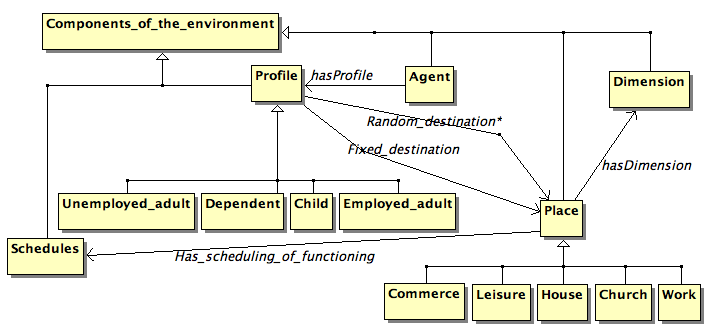
\includegraphics[width=150mm]{figuras/UEMontology.png}
  \caption{Modelo de ambiente urbano \cite{paiva2005ontology}.}
  \label{fig:UEM}
\end{figure}

Assim, \emph{Profile} permite definir locais usuais (fixos) e eventuais
(randômicos). Esses locais são definidos pelo conceito \emph{Place} que contêm
uma descrição de sua capacidade (quantidade máxima de atores), dimensão
(acessível por relação) e horário de funcionamento (acessível por relação). O
conceito de \emph{Dimension} guarda a posição dos eixos X e Y, altura e
largura. Finalmente, o último \emph{Schedules} possui o horário de abertura e
fechamento, intervalo de entrada e tempo médio de permanência. %A decisão de
%para onde determinado agente irá é feita pelo ambiente através do conhecimento
%do perfil do ator, dessa forma, é possível carregar uma maior quantidade de
%atores.

Este trabalho pode ser pensado como a descrição da mentalidade dos personagens
através da descrição dos atores em um ambiente urbano em sua vida normal. O
foco da ontologia seguinte é o humano virtual propriamente dito. Assim, as
informações gerais do personagem, como, por exemplo, raça, cor e outros são
armazenadas na ontologia descrita visando uma descrição completa e reusável.
A Figura~\ref{fig:OVH} apresenta os principais conceitos da ontologia
desenvolvida por \citet{Gutierrez:2007:OVH:1229160.1229164}.

O conceito principal definido na ontologia é o \emph{Virtual Human}. O modelo
pode ser utilizado para representar pessoas virtuais ou reais. Humanos
(virtuais) podem serem descritos por \emph{Structural Descriptors} e
\emph{Morphological Descriptors}. Neste último são guardados os dados gerais
do personagem, por exemplo idade, sexo, altura, peso e etc. No outro conceito,
\emph{Structural Descriptors} é uma abstração que define os pontos de entrada
para uma variedade de descritores utilizados para explicar como o humano
virtual esta organizado. A organização por esqueleto foi o foco e se baseou na
especificação H-Anim\footnote{É uma especificação que descreve quantidade,
posição e rotação dos ossos para tentar padronizar os modelos.
Veja \url{http://www.h-anim.org/}.}. Como pode ser visto, é possível guardar
informações de geometria, textura e outras informações.

\begin{figure}[t]
  \centering
    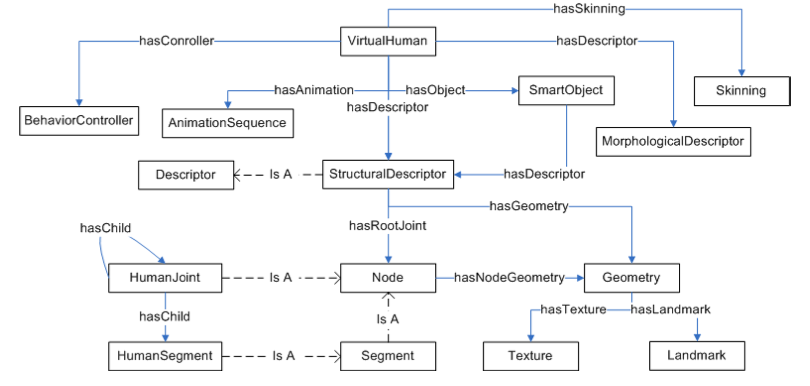
\includegraphics[width=150mm]{figuras/gutierrezVH.png}
  \caption{Ontologia de Humano Virtual \cite{Gutierrez:2007:OVH:1229160.1229164}.}
  \label{fig:OVH}
\end{figure}

Assim, o corpo humano consiste de um número de \emph{Segment} (por exemplo,
pé, mão e etc) que são conectados por \emph{Node}. Cada \emph{Node} pode
conter outros e, também, um \emph{Segment}. Além disso, ela pode ser animada
de duas formas. A primeira é através de uma animação sequencial pre-gravada
representada pelo conceito \emph{Animation Sequence} e a segunda é utilizando
o conceito de \emph{Behavioral Controller}. Esse último pode ser utilizado
para embutir um comportamento mais autônomo. Por fim, o conceito de
\emph{Smart Object} representa todos os objetos que podem ser manipulados por
um humano virtual.

\citet{grimaldo2006ontology} descreveu uma ontologia de ambiente inteligente
onde os agentes podem interagir, isto é, descreve o ambiente e permite
obter o estado do mundo. Por exemplo, a garrafa esta sobre a mesa ou o copo é
segurado pelo garçom. Além disso, em \citet{muller2010amabid} foi feita uma
ontologia para descrever atores implementados em \jason\footnote{Ver
\url{http://jason.sf.net} para mais detalhes.} de uma visão literária. Ambos
os trabalhos possuem uma visão simplificada dos atores por não serem o foco
principal de seus trabalhos.

%2345678901234567890123456789012345678901234567890123456789012345678901234567890
